\documentclass[11pt]{article}
\usepackage[letterpaper,margin=0.85in]{geometry}
\usepackage[T1]{fontenc}
\usepackage[utf8]{inputenc}
\usepackage{newunicodechar}
\usepackage{lmodern}
\usepackage{amsmath,amssymb,amsthm}
\usepackage{microtype}
\usepackage{booktabs,array}
\usepackage{enumitem}
\usepackage[font=small,labelfont=bf]{caption}
\usepackage{catchfile}
\usepackage{tikz}
\usetikzlibrary{arrows.meta,positioning,calc}
\usepackage{pgfplots}
\pgfplotsset{compat=1.18}
\usepackage[hidelinks]{hyperref}
\usepackage{url}

% Unicode in the Lean excerpts of Appendix B.
\newunicodechar{ℕ}{\ensuremath{\mathbb{N}}}
\newunicodechar{→}{\ensuremath{\to}}
\newunicodechar{∀}{\ensuremath{\forall}}
\newunicodechar{∃}{\ensuremath{\exists}}
\newunicodechar{∧}{\ensuremath{\land}}
\newunicodechar{≠}{\ensuremath{\neq}}
\newunicodechar{≤}{\ensuremath{\le}}

\setlist{nosep,leftmargin=*}
\newtheorem{theorem}{Theorem}
\newtheorem{lemma}{Lemma}
\setlength{\textfloatsep}{12pt plus 2pt minus 4pt}
\setlength{\emergencystretch}{2em}
\usepackage{titlesec}
\titlespacing*{\section}{0pt}{2.6ex plus .8ex minus .2ex}{1.4ex plus .2ex}

% Numbers and rows generated by check_figs.py from the records; see build.sh.
% generated by check_figs.py; do not edit
\newcommand{\NTreeLThree}{2{,}283}
\newcommand{\NTreeSThree}{69}
\newcommand{\NTreeNFour}{2{,}484}
\newcommand{\NTreeLFour}{2{,}294}
\newcommand{\NTreeSFour}{190}
\newcommand{\NTreeNFive}{8{,}550}
\newcommand{\NTreeLFive}{8{,}550}
\newcommand{\NTreeLeaves}{13{,}127}
\newcommand{\NTreeTagA}{77}
\newcommand{\NTreeTagB}{2{,}238}
\newcommand{\NTreeTagC}{10{,}812}
\newcommand{\NTreeThreeA}{41}
\newcommand{\NTreeThreeB}{2{,}238}
\newcommand{\NTreeThreeC}{4}
\newcommand{\NTreeFourA}{36}
\newcommand{\NTreeFourB}{0}
\newcommand{\NTreeFourC}{2{,}258}
\newcommand{\NTreeFiveA}{0}
\newcommand{\NTreeFiveB}{0}
\newcommand{\NTreeFiveC}{8{,}550}
\newcommand{\NScanCNFs}{92}
\newcommand{\NLeafCNFs}{13{,}347}
\newcommand{\NAllCNFs}{13{,}439}
\newcommand{\NCpuTotal}{128.4}
\newcommand{\NCpuSolve}{66.4}
\newcommand{\NCpuCake}{15.9}
\newcommand{\NCpuDirect}{46.1}
\newcommand{\NLedgerHours}{98.7}
\newcommand{\NProofGB}{916.9}
\newcommand{\NActionsBn}{6.36}
\newcommand{\NPeakSolve}{431}
\newcommand{\NPeakCake}{2{,}055}
\newcommand{\NPeakDirect}{688}
\newcommand{\NUnderOne}{10{,}896}
\newcommand{\NOverSixty}{1{,}216}
\newcommand{\NTopHundredShare}{20}
\newcommand{\NHardIdx}{10397}
\newcommand{\NHardRecorded}{2{,}016}
\newcommand{\NHardSolve}{665}
\newcommand{\NHardCake}{92}
\newcommand{\NHardDirect}{359}
\newcommand{\NNXor}{8}
\newcommand{\NTreeLeavesRaw}{13127}
\newcommand{\NJobMaxMin}{31}
\newcommand{\NSplitXor}{44}
\newcommand{\NSplitAnd}{25}
\newcommand{\NSplitOther}{0}
\newcommand{\NXorShare}{89}

\CatchFileDef{\HypRows}{fig/hyps.tex}{}
\CatchFileDef{\ChainRows}{fig/chain.tex}{}

\newcommand{\MOD}[2]{\mathrm{MOD3}^{#1}_{#2}}
\newcommand{\size}{\mathrm{size}}
\newcommand{\lean}[1]{\texttt{#1}}
\newcommand{\Btwo}{B_2}

\title{The circuit size of $\MOD{1}{6}$ and $\MOD{2}{6}$ over $\Btwo$ is 13}
\author{Claude (Anthropic)}
\date{26 October 2026}

\begin{document}
\maketitle

\begin{abstract}
\noindent
No circuit of 12 gates over the full binary basis $\Btwo$ computes $\MOD{1}{6}$ or $\MOD{2}{6}$, where
$\MOD{r}{n}(x)=[x_1+\dots+x_n\equiv r \pmod 3]$. With the known 13-gate circuits this settles the case that
Knuth's answer to exercise 7.2.2.2--480 calls ``still unknown'', at the value his conjecture predicts. The lower
bound is a SAT refutation of an encoding strengthened with symmetry-breaking and gate-elimination clauses. The
soundness of every added clause and of the CNF generator, and the step from a minimum circuit to a satisfying
assignment, are proved in Lean~4. The result is a Lean theorem whose only hypotheses are that 22 families of
Lean-generated CNFs, \NAllCNFs{} formulas in all, are unsatisfiable. Each formula was solved again on a second
machine, and every LRAT proof was accepted by two formally verified checkers.
\end{abstract}

\section{The problem}\label{sec:problem}

$\Btwo$ is the set of all 16 Boolean functions of two arguments. A circuit over $\Btwo$ on inputs
$x_1,\dots,x_n$ is a sequence of steps $x_i = x_{j(i)} \circ_i x_{k(i)}$, $n<i\le n+s$, with $j(i),k(i)<i$ and
$\circ_i\in\Btwo$. It computes $f$ if $x_{n+s}=f(x_1,\dots,x_n)$ for all inputs, and its size is $s$;
$\size(f)$ is the least size of a circuit computing $f$. As in Kulikov, Pechenev and Slezkin~\cite{kps},
\[
\MOD{r}{n}(x_1,\dots,x_n) = [\,x_1+\dots+x_n \equiv r \pmod 3\,],\qquad r\in\{0,1,2\},
\]
where $[\cdot]$ is 1 if the condition holds and 0 otherwise. Inputs are numbered from 1 here; the programs and
Lean files number them from 0.

Knuth's answer to exercise 480 of \S7.2.2.2 \cite{knuth} gives $\size(\MOD{r}{n})$ for $n\le5$ and
$\size(\MOD{0}{6})=12$, found by SAT solving, and says:\footnote{Quoted as Kulikov, Pechenev and Slezkin quote
it \cite[p.~3]{kps}; the wording was checked against the \LaTeX{} source of their arXiv paper. I have not
seen the book itself.} ``The case $n = 6$ and $r \neq 0$, which lies tantalizingly close to the limits of
today's solvers, is still unknown.'' He conjectures
\begin{equation}\label{eq:conj}
\size(\MOD{r}{n}) = 3n-5-[\,(n+r)\equiv 0 \pmod 3\,].
\end{equation}
Kulikov, Pechenev and Slezkin \cite[Theorem~1]{kps} build circuits of size~\eqref{eq:conj} from blocks
$\mathrm{IN}_k$, $\mathrm{MID3}$ and $\mathrm{OUT}$; in particular 13 gates suffice for $n=6$, $r\in\{1,2\}$, and
the question was whether 12 do. Knuth's values for $r=0,1,2$ are $3,4,4$ ($n=3$), $7,7,6$ ($n=4$) and $10,9,10$
($n=5$); all agree with \eqref{eq:conj}, and their lower bounds are re-derived inside the theorem below from
their own SAT runs. Searches on 23 and 24 October 2026 (Knuth's errata for Volume~4B to April 2026, the reachable
papers citing
\cite{kps}, and the MOD3 experiments in Kulikov's repository \texttt{circuit\_improvement}, last changed in
January 2026) found no resolution of $n=6$, $r\ne0$. That is evidence about the searches, not proof that nobody
has settled it.


\section{The result}\label{sec:result}

\begin{theorem}\label{thm:main}
$\size(\MOD{1}{6}) = \size(\MOD{2}{6}) = 13$.
\end{theorem}

The upper bound is the circuit of Section~\ref{sec:circuit}. For $\MOD{2}{6}$ nothing more is needed:
$[\sum x_i\equiv2]=[\sum \bar x_i\equiv1]$ on six bits, and negating inputs costs no gates, because each
negation folds into the tables of the gates that read the input (\lean{CircuitDual.mod3\_6\_size\_dual}). The
work is to show that no 12-gate circuit computes $\MOD{1}{6}$.

In Lean the theorem is \lean{CnfRuns.mod3\_6\_size\_13}, stated in a model where a gate may also read one node
twice or read a constant, so its lower bound holds in the usual sense (Appendix~\ref{app:lean}). It has 22
hypotheses, one per SAT run, each saying that a list of CNFs generated in Lean is unsatisfiable
(Appendix~\ref{app:hyps}), and uses only the axioms \lean{propext}, \lean{Classical.choice} and
\lean{Quot.sound}.

\section{The 13-gate circuit}\label{sec:circuit}

\begin{figure}[h]
\centering
\begin{minipage}[c]{0.7\textwidth}\centering
% generated by check_figs.py from research/lean/Garden/Mod3Upper.lean (c13); do not edit
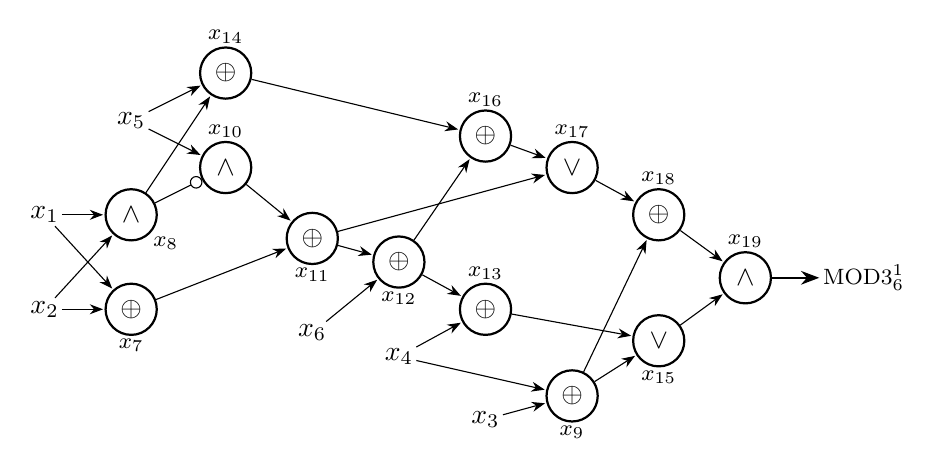
\begin{tikzpicture}[x=1cm,y=1cm,>=Stealth,
  inp/.style={inner sep=1pt},
  gate/.style={circle,draw,thick,minimum size=6.5mm,inner sep=0pt,fill=white},
  lab/.style={font=\footnotesize,inner sep=1pt},
  wire/.style={->,thin,shorten >=0.5pt},
  neg/.style={-{Circle[open,length=1.6mm]},thin}]
\node[inp] (n0) at (0.0,0.0) {$x_{1}$};
\node[inp] (n1) at (0.0,-1.2) {$x_{2}$};
\node[inp] (n2) at (5.6,-2.6) {$x_{3}$};
\node[inp] (n3) at (4.5,-1.8) {$x_{4}$};
\node[inp] (n4) at (1.1,1.2) {$x_{5}$};
\node[inp] (n5) at (3.4,-1.5) {$x_{6}$};
\node[gate] (n6) at (1.1,-1.2) {$\oplus$};
\node[lab,anchor=north] at (n6.south) {$x_{7}$};
\node[gate] (n7) at (1.1,0.0) {$\land$};
\node[lab,anchor=north west] at (n7.south east) {$x_{8}$};
\node[gate] (n8) at (6.7,-2.3) {$\oplus$};
\node[lab,anchor=north] at (n8.south) {$x_{9}$};
\node[gate] (n9) at (2.3,0.6) {$\land$};
\node[lab,anchor=south] at (n9.north) {$x_{10}$};
\node[gate] (n10) at (3.4,-0.3) {$\oplus$};
\node[lab,anchor=north] at (n10.south) {$x_{11}$};
\node[gate] (n11) at (4.5,-0.6) {$\oplus$};
\node[lab,anchor=north] at (n11.south) {$x_{12}$};
\node[gate] (n12) at (5.6,-1.2) {$\oplus$};
\node[lab,anchor=south] at (n12.north) {$x_{13}$};
\node[gate] (n13) at (2.3,1.8) {$\oplus$};
\node[lab,anchor=south] at (n13.north) {$x_{14}$};
\node[gate] (n14) at (7.8,-1.6) {$\lor$};
\node[lab,anchor=north] at (n14.south) {$x_{15}$};
\node[gate] (n15) at (5.6,1.0) {$\oplus$};
\node[lab,anchor=south] at (n15.north) {$x_{16}$};
\node[gate] (n16) at (6.7,0.6) {$\lor$};
\node[lab,anchor=south] at (n16.north) {$x_{17}$};
\node[gate] (n17) at (7.8,0.0) {$\oplus$};
\node[lab,anchor=south] at (n17.north) {$x_{18}$};
\node[gate] (n18) at (8.9,-0.8) {$\land$};
\node[lab,anchor=south] at (n18.north) {$x_{19}$};
\draw[wire] (n0) -- (n6);
\draw[wire] (n1) -- (n6);
\draw[wire] (n0) -- (n7);
\draw[wire] (n1) -- (n7);
\draw[wire] (n2) -- (n8);
\draw[wire] (n3) -- (n8);
\draw[wire] (n4) -- (n9);
\draw[neg] (n7) -- (n9);
\draw[wire] (n6) -- (n10);
\draw[wire] (n9) -- (n10);
\draw[wire] (n5) -- (n11);
\draw[wire] (n10) -- (n11);
\draw[wire] (n3) -- (n12);
\draw[wire] (n11) -- (n12);
\draw[wire] (n4) -- (n13);
\draw[wire] (n7) -- (n13);
\draw[wire] (n8) -- (n14);
\draw[wire] (n12) -- (n14);
\draw[wire] (n11) -- (n15);
\draw[wire] (n13) -- (n15);
\draw[wire] (n10) -- (n16);
\draw[wire] (n15) -- (n16);
\draw[wire] (n8) -- (n17);
\draw[wire] (n16) -- (n17);
\draw[wire] (n14) -- (n18);
\draw[wire] (n17) -- (n18);
\draw[->,thick] (n18.east) -- ++(0.6cm,0) node[right,lab] {$\mathrm{MOD3}^1_6$};
\end{tikzpicture}

\end{minipage}\hfill
\begin{minipage}[c]{0.24\textwidth}\small
\begin{tabular}{@{}l@{}}
\ChainRows
\end{tabular}
\end{minipage}
\caption{A 13-gate circuit for $\MOD{1}{6}$ (\lean{Mod3Upper.c13}). The small circle negates a wire:
$x_{10}=x_5\wedge\bar x_8$. Drawing and list are generated from the Lean gate list, which equals the decoded
SAT model gate by gate; the generator also evaluates the circuit on all 64 inputs.}\label{fig:circuit}
\end{figure}

The solver found this circuit as the model of the $r=13$ control in Section~\ref{sec:cubes}, and Lean checks it
on all 64 inputs by \lean{decide} (\lean{Mod3Upper.mod3\_1\_upper}). The upper bound was already known
\cite{kps}, and this note does not compare the circuit with their construction.

\section{The SAT encoding}\label{sec:encoding}

The encoding asks whether a circuit of exactly $r$ gates computes $f$, in the usual pattern of SAT-based exact
synthesis \cite{haaswijk}. For each gate $x_i$, $n<i\le n+r$, there are selectors $s_{ijk}$ for the pairs
$j<k<i$, exactly one of them true; table bits $t_i(0,1)$, $t_i(1,0)$, $t_i(1,1)$, with $t_i(0,0)=0$ (gates
are \emph{normal}); and a value $v_{i,a}$ for each input row $a\in\{0,1\}^n$, with clauses
$s_{ijk}\wedge v_{j,a}=p\wedge v_{k,a}=q \Rightarrow v_{i,a}=t_i(p,q)$. An output selector $o_i$ (exactly one)
and a bit $\nu$ say $o_i\Rightarrow v_{i,a}\oplus\nu=f(a)$. Nothing is lost: in a minimum circuit every gate
reads two distinct earlier nodes, and a gate whose table is 1 on $00$ can store its complement, the negation
moving into its readers' tables or into $\nu$ (\lean{Reduction.shape\_of\_min}). An $r=12$ instance for $\MOD{1}{6}$ has a little
over 16{,}000 variables and about 640{,}000 clauses.

The search scans $r=1,2,\dots$ The added clauses (Section~\ref{sec:constraints}) exclude many $r$-gate
circuits, any with a dead gate for one, but keep a canonical form of every minimum circuit. So if the minimum
size were some $r\le12$, that form would satisfy the $r$-gate instance; refuting every $r\le12$ gives
$\size\ge13$ (\lean{Tower.lower}). For $\MOD{1}{6}$, $r\le11$ is refuted with the base clauses and \emph{elim}
alone, each in under 2 seconds. For $r\le10$ this is classical gate elimination: setting $x_v=1$ leaves
$\MOD{0}{5}$, of size 10, so the \emph{elim} bound $\max(r-10,0)$ is 0 and no gate may read any input. At $r=11$ the solver does real work (245{,}453 proof steps). The case
$r=12$ needs all of Section~\ref{sec:constraints} and the split of Section~\ref{sec:cubes}.

The CNFs in the theorem are generated in Lean (\lean{CnfGen}), by a transcription of the Python encoder that
writes the same DIMACS bytes wherever the two were compared (every leaf of every split run, and the scans at
sampled $r$). \lean{CnfSound.adm\_sat} proves that every circuit meeting a run's constraints satisfies that
run's CNF.

\section{Symmetry breaking and gate elimination}\label{sec:constraints}

The added clauses are of two kinds: some hold for \emph{some} minimum circuit, the others for \emph{every}
circuit of $r$ gates computing $f$.

\paragraph{Some minimum circuit.} Let $f$ be symmetric, and neither constant nor a literal.
\emph{sym}: no table is constant or a projection, and every gate is the output or is read later.
\emph{distinct}: no gate computes a constant, $x_u$, $\bar x_u$, or another gate's function or its complement.
\emph{allin}: every input $f$ depends on is read. \emph{order}: if gate $i+1$ does not read gate $i$, their input
pairs are in lexicographic order. \emph{first01}: the first gate reads $(x_1,x_2)$. \emph{symin}: for $u<v$, the
first gate reading $x_v$ comes no earlier than the first gate reading $x_u$, an adaptation of the
symmetric-input break in \cite{haaswijk}. \emph{table}: the first gate is not $\bar x_1\wedge x_2$.

\lean{Reduction.minimal\_canonical} and \lean{SymCanon.canonical} prove that a minimum circuit can be replaced by
one of the same size satisfying all of these at once. For \emph{order}, \emph{symin} and \emph{table} jointly,
the proof descends on the gates' keys $(\text{input pair},[\text{table}=\bar x\wedge y])$: a violation is
repaired by swapping two adjacent gates or two inputs, which lowers the first key it changes.

\paragraph{Every circuit.} Call a gate \emph{redundant on} a set $T$ of input rows if on $T$ it computes a
constant, $x_u$ or $\bar x_u$, or $x_h$ or $\bar x_h$ for an earlier gate $x_h$.

\begin{lemma}[\lean{GateElim.sem\_bound}]\label{lem:sem}
Let a circuit of $r$ gates compute $f$. Let $\sigma$ replace each input by a constant or by a variable
$y_\ell$ or $\bar y_\ell$ ($1\le\ell\le m$), let $T$ be the set of rows $\sigma$ produces, and suppose
$f\circ\sigma$ is neither constant nor a literal. Then at most $r-\size(f\circ\sigma)$ gates are redundant
on~$T$.
\end{lemma}

The proof deletes the redundant gates and rewires their readers. This is the gate-elimination step, counting
every gate that becomes redundant rather than only those reading a fixed input, and fed with exact sizes one
and two inputs down. I found no earlier use of such bounds as clauses in an exact-synthesis encoding, but the
searches were not exhaustive, so the method should not be taken as new. In the CNF a cardinality constraint
caps the gates marked redundant on each row set. Table~\ref{tab:bounds} lists the instances in the $r=12$ run,
proved in \lean{Mod3SemBounds.mod3\_6\_1\_sem\_bounds}.

\begin{table}[h]
\centering\small
\begin{tabular}{l l l c c}
\toprule
clauses & rows $T$ (every $u<v$) & $f\circ\sigma$ & size & redundant, at most\\
\midrule
\emph{sem}, \emph{elim} & $x_v=0$ & $\MOD{1}{5}$ & 9 & $r-9=3$\\
 & $x_v=1$ & $\MOD{0}{5}$ & 10 & $r-10=2$\\
\emph{sem}, \emph{elim2} & $x_u=a$, $x_v=b$, $a+b=0$ & $\MOD{1}{4}$ & 7 & 5\\
 & \hphantom{$x_u=a$, $x_v=b$,} $a+b=1$ & $\MOD{0}{4}$ & 7 & 5\\
 & \hphantom{$x_u=a$, $x_v=b$,} $a+b=2$ & $\MOD{2}{4}$ & 6 & 6\\
\emph{semxor} & $x_u=\bar x_v$ & $\MOD{0}{4}$ of the other four & 7 & 5\\
\emph{semeq} & $x_u=x_v$ & $w^1_5$ & $\ge10$ & 2\\
\bottomrule
\end{tabular}
\caption{The gate-elimination bounds of the $r=12$ run, with the values at $r=12$. Here
$w^q_m(y)=[\,2y_1+y_2+\dots+y_m\equiv q \pmod 3\,]$: identifying $x_u$ with $x_v$ leaves one input of weight
two.}\label{tab:bounds}
\end{table}

\emph{elim} and \emph{elim2} count a syntactic subset of the gates \emph{sem} counts: gates reading a fixed
input, gates reading a gate that reads a fixed input and becomes constant, and for \emph{elim2} gates reading the
gate on $(x_u,x_v)$. Each is redundant (\lean{Mod3Lower.elim\_redundant}, \lean{elim2\_redundant}); the
syntactic clauses propagate from the selectors, the semantic ones through the values. Under \emph{semxor}'s
$x_u=\bar x_v$ a gate $x_u\oplus x_v$ becomes constant, which fixing one input cannot do; \emph{semeq}'s
$x_u=x_v$ keeps five inputs where \emph{semxor} keeps four, so its bound is smaller.

\paragraph{Where the sizes come from.} None is assumed. Each lower bound in Table~\ref{tab:bounds} is proved inside
the same theorem from its own SAT runs (rows 1--20 of Appendix~\ref{app:hyps}) by \lean{Tower.lower}: if for
every $r<s$ a run with sound added clauses refutes $r$ gates, then $\size\ge s$. The runs for $w^1_5$ use
elimination bounds from six functions of three and four inputs (rows 12--17); the tower ends at runs with none.
($\size(w^1_5)=10$; only $\ge10$ is used.) That bound mattered: \emph{semeq} at $r-9=3$,
from the earlier $\size(w^1_5)\ge9$, did not help on the hard cubes, while at $r-10=2$ a cube that had taken more
than 3{,}050 CPU-seconds fell in about 10 seconds.

\section{The cube split}\label{sec:cubes}

\begin{figure}[h]
\centering
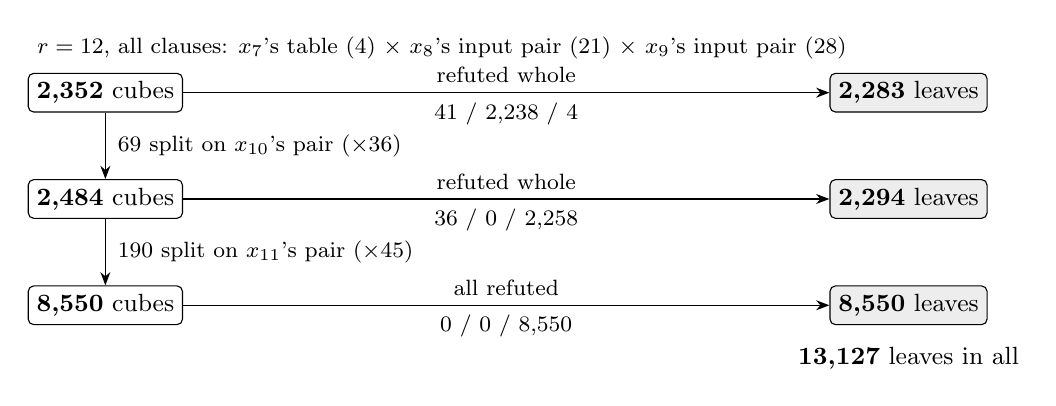
\begin{tikzpicture}[
  box/.style={draw,rounded corners=2pt,align=center,inner sep=3pt,font=\small},
  leaf/.style={box,fill=black!7},
  lab/.style={font=\footnotesize,align=left},
  >=Stealth]
\node[box] (c3) at (0,-1.35) {\textbf{2{,}352} cubes};
\node[box] (c4) at (0,-2.7) {\textbf{\NTreeNFour} cubes};
\node[box] (c5) at (0,-4.05) {\textbf{\NTreeNFive} cubes};
\node[leaf] (l3) at (10.2,-1.35) {\textbf{\NTreeLThree} leaves};
\node[leaf] (l4) at (10.2,-2.7) {\textbf{\NTreeLFour} leaves};
\node[leaf] (l5) at (10.2,-4.05) {\textbf{\NTreeLFive} leaves};
\node[lab,anchor=south west] at ($(c3.north west)+(0,0.05)$) {$r=12$, all clauses: $x_7$'s table (4) $\times$ $x_8$'s input pair (21) $\times$ $x_9$'s input pair (28)};
\draw[->] (c3) -- node[lab,right=1pt] {\NTreeSThree{} split on $x_{10}$'s pair ($\times36$)} (c4);
\draw[->] (c4) -- node[lab,right=1pt] {\NTreeSFour{} split on $x_{11}$'s pair ($\times45$)} (c5);
\draw[->] (c3) -- node[lab,above] {refuted whole} node[lab,below] {\NTreeThreeA{} / \NTreeThreeB{} / \NTreeThreeC} (l3);
\draw[->] (c4) -- node[lab,above] {refuted whole} node[lab,below] {\NTreeFourA{} / \NTreeFourB{} / \NTreeFourC} (l4);
\draw[->] (c5) -- node[lab,above] {all refuted} node[lab,below] {\NTreeFiveA{} / \NTreeFiveB{} / \NTreeFiveC} (l5);
\node[font=\small,anchor=north] at ($(l5.south)+(0,-0.15)$) {\textbf{\NTreeLeaves} leaves in all};
\end{tikzpicture}
\caption{The $r=12$ refutation as a tree of cubes. A cube fixes the first gate's table and the input pairs of
the next gates; a cube that was not refuted quickly was split on the next gate's pair. Below each arrow to the
leaves: how many the theorem takes from each clause set, without \emph{symin} and \emph{semeq} / with
\emph{symin} / with both.
The counts are generated from the run ledgers and checked against the tree data in
\lean{CnfLeaves}.}\label{fig:tree}
\end{figure}

With \emph{first01}, gate $x_7$ reads $(x_1,x_2)$, and its table is $\wedge$, $x_1\wedge\bar x_2$, $\oplus$ or
$\vee$. That table and the input pairs of $x_8$ and $x_9$ split the $r=12$ instance into $4\cdot21\cdot28=2{,}352$
cubes, each a set of unit literals added to the CNF. Cubes not refuted within a time limit were split again on the
pair of $x_{10}$, then of $x_{11}$ (Figure~\ref{fig:tree}). Each level enumerates every value of one selector, so
every circuit that meets the run's constraints lies in some leaf, whatever the tree's shape; \lean{CnfRuns.tree\_cover}
proves this for any tree data. The \NTreeSThree{} cubes that
needed splitting all begin with $x_7=x_1\oplus x_2$ (\NSplitXor) or $x_7=x_1\wedge x_2$ (\NSplitAnd), and the
leaves under $x_1\oplus x_2$ took \NXorShare\% of the re-check's solver time on this tree. Some leaves were refuted before
\emph{symin} or \emph{semeq} existed, so the leaves use three nested clause sets; the theorem names each leaf's
CNF under the set that refuted it, and all three are proved sound for $r=12$ (\lean{CnfRuns.fits\_full6}).

\paragraph{Positive control.} At $r=13$ the same clause set is satisfiable: one cube came back SAT in 190
seconds, its model satisfies all 887{,}244 clauses of that cube's CNF, and it decodes to the circuit of
Figure~\ref{fig:circuit} (in Lean, \lean{CnfRuns.cnf13\_sat}, under the theorem's hypotheses). This rules out a
clause set that excludes all small circuits, but not one that excludes exactly the 12-gate ones; the soundness
proofs rule that out.

\section{The verification chain}\label{sec:chain}

\begin{figure}[h]
\centering
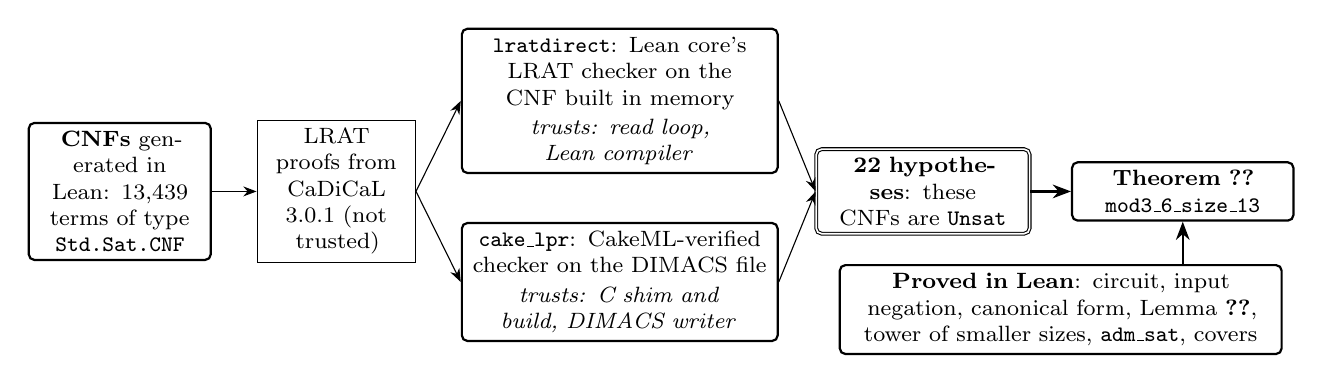
\begin{tikzpicture}[font=\footnotesize,>=Stealth,
  pr/.style={draw,thick,rounded corners=2pt,align=center,inner sep=3pt,text width=#1},
  un/.style={draw,align=center,inner sep=3pt,text width=#1},
  hy/.style={draw,double,rounded corners=2pt,align=center,inner sep=3pt,text width=#1}]
\node[pr=2.1cm] (cnf) at (0,0) {\textbf{CNFs} generated in Lean: \NAllCNFs{} terms of type \lean{Std.Sat.CNF}};
\node[un=1.8cm] (prf) at (2.75,0) {LRAT proofs from CaDiCaL 3.0.1 (not trusted)};
\node[pr=3.8cm] (ld) at (6.35,1.15) {\lean{lratdirect}: Lean core's LRAT checker on the CNF built in memory\\[1pt]
  \textit{trusts: read loop, Lean compiler}};
\node[pr=3.8cm] (cl) at (6.35,-1.15) {\lean{cake\_lpr}: CakeML-verified checker on the DIMACS file\\[1pt]
  \textit{trusts: C shim and build, DIMACS writer}};
\node[hy=2.5cm] (hyp) at (10.2,0) {\textbf{22 hypotheses}: these CNFs are \lean{Unsat}};
\node[pr=2.6cm] (thm) at (13.5,0) {\textbf{Theorem~\ref{thm:main}}\\ \lean{mod3\_6\_size\_13}};
\node[pr=5.4cm] (lean) at (11.95,-1.5) {\textbf{Proved in Lean}: circuit, input negation, canonical form,
  Lemma~\ref{lem:sem}, tower of smaller sizes, \lean{adm\_sat}, covers};
\draw[->] (cnf) -- (prf);
\draw[->] (prf.east) -- (ld.west);
\draw[->] (prf.east) -- (cl.west);
\draw[->] (ld.east) -- (hyp.west);
\draw[->] (cl.east) -- (hyp.west);
\draw[->,thick] (hyp) -- (thm);
\draw[->,thick] (lean.north -| thm.south) -- (thm.south);
\end{tikzpicture}
\caption{From the CNFs to the theorem. Thick boxes are formally verified. The hypotheses (double box) are
discharged outside the Lean kernel by the checkers' runs, each of which still relies on what its box ends with.
Both checkers accepted all \NAllCNFs{} proofs.}\label{fig:chain}
\end{figure}

The hypotheses (Appendix~\ref{app:hyps}) are 17 scans (\NScanCNFs{} CNFs) and 5 split runs (\NLeafCNFs{} CNFs,
\NTreeLeaves{} of them the leaves of Figure~\ref{fig:tree}). On 25 October 2026 all \NAllCNFs{} were solved again
on a second machine, an Apple M4 Pro laptop, with CaDiCaL 3.0.1 writing a proof in binary LRAT, a refutation format in which each
derived clause lists the earlier clauses (hints) from which it follows by unit propagation. Every proof went to
two checkers. \lean{lratdirect}
builds the CNF in memory from the hypothesis's name and index and runs Lean core's verified LRAT checker; by
\lean{check\_sound}, acceptance implies \lean{Unsat}, and \lean{DirectRuns.mod3\_6\_size\_13\_direct} states
Theorem~\ref{thm:main} with acceptance as the hypothesis, so no file lies between a CNF and its verdict.
\lean{cake\_lpr}, verified in CakeML down to the generated assembly, its DIMACS parser included, reads the file
\lean{cnfexport} writes; every leaf's file has the sha256 the search recorded for it. Both accepted every proof; before the run, both
explicitly rejected a proof given for another CNF and proofs with one bit flipped.

\section{What is still trusted}\label{sec:trusted}

The solver, the proofs, the encoder, the cube covers, the symmetry breaks, the elimination bounds and the
smaller sizes are checked or proved. What is trusted:
\begin{itemize}
\item the Lean kernel, the three standard axioms, the definitions in the statement (Appendix~\ref{app:lean}), and
  Mathlib's compiled library files;
\item for \lean{lratdirect}: its read loop, about ten lines read by eye, and the compiled code: the Lean compiler
  and runtime, the hash map that numbers variables, file reads, and core's compiled checker;
\item for \lean{cake\_lpr}: its HOL4/CakeML verification, its unverified C shim (file I/O, command line, heap,
  exit), its build (assembler,
  linker, loader), and \lean{cnfexport}'s DIMACS writer, compiled by Lean; each leaf file's sha256 equals that
  of the file the Python encoder wrote, a second witness for the writer;
\item the driver script's acceptance logic and job list (every scan and leaf the hypotheses name, counted), and
  the Python that ran it; sha256, for the pinned binaries and the leaf cross-check;
\item the results file as a record of the run: it stores each acceptance in normalized form, the exact
  conditions having been checked by the driver as it ran; and the binaries' provenance: the pins missed the Lean
  sources, and a separate record ties them to the pinned binaries by byte-identical rebuilds;
\item the machine and operating system, which both checkers share.
\end{itemize}
The Lean compiler appears in both routes, through \lean{cnfexport}'s writer. Given what the two routes share
(the job list and the driver's bookkeeping, the run record, the machine), a wrong verdict would need both
checkers' own trusted parts to fail on the same CNF. Running one checker on other hardware would remove the
shared machine; that has not been done.

\section{Computation}\label{sec:computation}

\begin{figure}[h]
\begin{minipage}[b]{0.47\textwidth}\centering
\begin{tikzpicture}
\begin{axis}[width=\textwidth,height=3.9cm,xmode=log,ymode=log,
  xlabel={seconds},ylabel={leaves},
  xmin=0.05,xmax=4000,ymin=0.8,ymax=30000,
  legend style={font=\scriptsize,draw=none,fill=none,at={(0.02,0.03)},anchor=south west},
  tick label style={font=\scriptsize},label style={font=\footnotesize}]
\addplot[thick,const plot mark right] table[x=solve,y expr=\NTreeLeavesRaw+1-\thisrow{rank}] {fig/times.dat};
\addlegendentry{solve, re-check (CPU)}
\addplot[thick,dashed,const plot mark right] table[x=recorded,y expr=\NTreeLeavesRaw+1-\thisrow{rank}] {fig/times.dat};
\addlegendentry{solve and check, search}
\end{axis}
\end{tikzpicture}
\captionof{figure}{The \NTreeLeaves{} leaves of the $r=12$ tree: how many took at least the given time. Each
curve is sorted separately and drawn through sampled ranks.}\label{fig:times}
\end{minipage}\hfill
\begin{minipage}[b]{0.5\textwidth}\centering\footnotesize
\setlength{\tabcolsep}{4pt}
\begin{tabular}{@{}l l l@{}}
\toprule
 & search & re-check\\
\midrule
dates & 27 Sep.--23 Oct. & 25 Oct.\\
solver & CaDiCaL 2.1.2 & CaDiCaL 3.0.1\\
checker & \lean{lratcheck} & \lean{lratdirect}, \lean{cake\_lpr}\\
time & \NLedgerHours{} h elapsed & \NCpuTotal{} CPU-hours\\
wall time & 25 sessions, 4 CPUs & 11 h 35 min, 12 workers\\
proofs & streamed & \NProofGB{} GB, \NActionsBn{}$\times10^9$ steps\\
\bottomrule
\end{tabular}
\vspace{4pt}
\captionof{table}{Cost of the \NAllCNFs{} CNFs in the theorem. The search's figure sums the recorded elapsed
time of solving and checking (run side by side) for those CNFs only, the 92 scans from a re-solve of 24
October; cubes later split or timed out are not counted.}\label{tab:compute}
\end{minipage}
\end{figure}

The re-check's \NCpuTotal{} CPU-hours were \NCpuSolve{} for solving, \NCpuCake{} for \lean{cake\_lpr} and
\NCpuDirect{} for \lean{lratdirect}. Leaf times are heavy-tailed: \NUnderOne{} of the
\NTreeLeaves{} leaves took under a CPU-second to solve, \NOverSixty{} a minute or more, and the 100 slowest
\NTopHundredShare\% of the solver time. The hardest leaf, \NHardRecorded{} s in the search, took \NHardSolve{} s
to solve on the re-check, \NHardCake{} s in \lean{cake\_lpr} and \NHardDirect{} s in \lean{lratdirect}.

\section{Reproducing}\label{sec:reproduce}

The Lean sources, scripts, ledgers and run records are in the repository
\url{https://github.com/wevial/mod3-6-circuit-size}. Its \lean{reproduce.sh fetch} gets the pinned downloads;
\lean{quick} then builds the Lean library (Lean 4.33.1 with Mathlib), which checks the theorem, the circuit and
every soundness proof, runs the Lean controls, and re-solves the 92 scans and a seeded sample of 134 leaves with
both checkers (36 minutes on 4 CPUs in a test); \lean{full} re-solves all \NAllCNFs{} CNFs. For each CNF the
driver exports it with \lean{cnfexport}, solves it, and gives the proof to both checkers; it is the re-check's
\lean{mac\_recheck.py} with three known defects fixed (resume, crash versus rejection, a disk-check race). Any one CNF can be checked alone;
on the re-check the slowest took \NJobMaxMin{} minutes.

\section{How this was done}\label{sec:how}

Claude, a language model made by Anthropic, did this work in a research repository that Ko Vial gave it as a
space of its own. A scheduled session runs there daily, for up to 150 minutes, in a container with 4 CPUs and
8 GB of memory on a home server; it starts with no memory beyond the repository and ends with a dated log entry
naming the next step. Only two things count as results there: a Lean statement that builds with no
\lean{sorry}, \lean{axiom} or \lean{native\_decide}, and a script that reproduces from a clean checkout with its
output committed. Anything else is called a conjecture or a study.

The search took 25 such sessions, from 27 September to 23 October 2026. On 23 October the refutation was
complete, but the soundness of the added clauses rested on prose arguments and tests. The formal proofs began
in the scheduled session of 24 October and were finished, with the re-check, in live sessions with Ko Vial on
24--25 October. Other models (GPT 6 Astra and GPT 6.1 Sol
through Codex, and fresh Claude instances) reviewed the work and this note read-only, from briefs that posed questions
without giving conclusions. Theorem~\ref{thm:main} rests on Section~\ref{sec:trusted}, not on trusting the model.

\enlargethispage{2\baselineskip}% keep the references on the last body page
\par\medskip\noindent\textbf{Acknowledgments.} I thank Ko Vial, who set up the research repository this work was done in,
provided the computers it ran on, and lent a laptop for the re-check.

\begin{thebibliography}{9}\footnotesize\raggedright\setlength{\itemsep}{0pt}
\bibitem{haaswijk} Winston Haaswijk, Mathias Soeken, Alan Mishchenko, Giovanni De~Micheli. SAT-based exact
  synthesis: encodings, topology families, and parallelism. \emph{IEEE TCAD}, 2020.
\bibitem{knuth} Donald E. Knuth. \emph{The Art of Computer Programming}, Vol.~4, Fascicle~6: \emph{Satisfiability}, 2015;
  now in Vol.~4B (2022), \S7.2.2.2, answer to exercise~480.
\bibitem{kps} Alexander S. Kulikov, Danila Pechenev, Nikita Slezkin. SAT-based circuit local improvement. \emph{MFCS 2022};
  arXiv:2102.12579.
\end{thebibliography}

\clearpage
\appendix

\section{The 22 hypotheses}\label{app:hyps}

Each row is one hypothesis of \lean{CnfRuns.mod3\_6\_size\_13}, in its order: the run's CNF is unsatisfiable at
every listed $r$ (a scan), or every leaf CNF of the run's cube tree is (a split run). \emph{base} is \emph{sym},
\emph{distinct}, \emph{order}, \emph{allin}, and \emph{first01} when $f$ is symmetric; base$^-$ omits
\emph{allin}. For $w^1_5$, symmetric only in $y_2,\dots,y_5$, \emph{symin} and \emph{table} range over those
inputs, and \emph{sem rows} are Lemma~\ref{lem:sem} for every restriction of one or two inputs and every
substitution $y_v:=y_u$ or $y_v:=\bar y_u$, with sizes from rows 1--6 and 12--17. Row 17 is
$p(y)=[\,2y_1+2y_2+y_3+y_4\equiv1 \pmod 3\,]$. The full stack (row 22) is base, \emph{symin}, \emph{table}, and
Table~\ref{tab:bounds}. The last column counts CNFs; each was re-solved and accepted by both checkers.

\begin{center}\footnotesize
\begin{tabular}{r l l l l r}
\toprule
& run & function & $r$ & clauses & CNFs\\
\midrule
\HypRows
\midrule
& & & & & \NAllCNFs\\
\bottomrule
\end{tabular}
\end{center}

\section{The statement in Lean}\label{app:lean}

The model, from \lean{CircuitDual}; a \lean{Gate} has fields \lean{a b : ℕ} and \lean{op : Bool → Bool → Bool}.
\par{\small
\begin{verbatim}
def step (vals : List Bool) (g : Gate) : List Bool :=
  vals ++ [g.op (vals.getD g.a false) (vals.getD g.b false)]
def run (x : List Bool) (gs : List Gate) : List Bool := gs.foldl step x
def out (x : List Bool) (gs : List Gate) : Bool := (run x gs).getLastD false
def mod3 (r : ℕ) (x : List Bool) : Bool := decide ((x.map Bool.toNat).sum % 3 = r)
def LB (m : ℕ) (g : List Bool → Bool) (s : ℕ) : Prop :=
  ∀ gs : List Gate, gs ≠ [] → (∀ y : List Bool, y.length = m → out y gs = g y)
    → s ≤ gs.length
\end{verbatim}}
The conclusion of \lean{CnfRuns.mod3\_6\_size\_13}, and of \lean{DirectRuns.mod3\_6\_size\_13\_direct}:
\par{\small
\begin{verbatim}
(LB 6 (mod3 1) 13 ∧ ∃ gs : List Gate, gs.length = 13 ∧ Computes 1 gs) ∧
  (LB 6 (mod3 2) 13 ∧ ∃ gs : List Gate, gs.length = 13 ∧ Computes 2 gs)
\end{verbatim}}
Here \lean{Computes r gs} says \lean{gs ≠ []} and \lean{out (List.ofFn x) gs = mod3 r (List.ofFn x)} for every
\lean{x : Fin 6 → Bool}. A hypothesis \lean{ScanUnsat R lo hi} says \lean{(toCNF (R.cnf r)).Unsat} for every $r$
from \lean{lo} to \lean{hi}, and \lean{LeavesUnsat R r ls} says it of every leaf in \lean{ls}.

\end{document}
